\section{Component/SubComponent Classes}

The Component and SubComponent python classes represent the Component
and SubComponent C++ classes that are used to implement the simulation
models used in SST.  They are similar, and have similar APIs, but
SubComponents can only exist inside of Components.  Subsequently,
Components are instanced directly, but SubComponents are only
instanced through a Component or another SubComponent.


Figure~\ref{fig:component-structure} shows the main pieces of the
Component/SubComponent.

\begin{figure}[h]
  \centering
  \subfigure[Main structures of the Component and SubComponent objects]{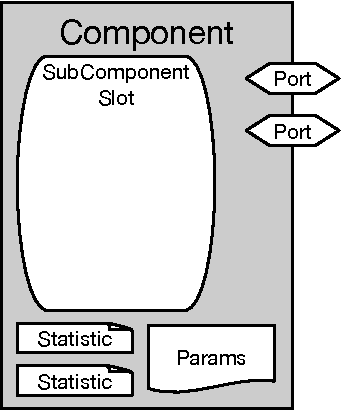
\includegraphics[width=0.3\textwidth]{figures/component-structure.pdf}} \hspace{1in}
  \subfigure[Component with SubComponents loaded, showing that SubComponents can be arbitrarily nested]{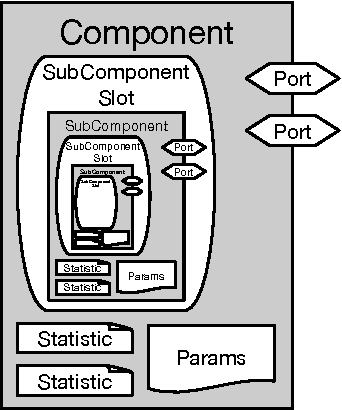
\includegraphics[width=0.3\textwidth]{figures/component-structure-with-subcomponent.pdf}}
  \caption[Structure of a Component]{Structure of a Component}
  \label{fig:component-structure}
\end{figure}

An instance of Component is created using:


\begin{functiondoc}{Component(name, element_type)}
  {Creates a new Component object.}

  \param{name} (type: string) name of the Component specified as
  string.  The name can be used to get a handle to the Component later
  in the python code.  The name is also available to the c++
  implementation of the Component

  \param{element\_type} (type: string) type of the Component in the
  lib.element format (for example, merlin.hr\_router) specified as a
  string

  \returns{Component object}
\end{functiondoc}

A SubComponent is created by calling setSubComponent() on either a
Component or SubComponent object.  Instancing a SubComponent in this
way creates a User SubComponent and allows the user to specify the
parameters and statistics directly on the SubComponent.  The name of
the SubComponent is automatically generated using the name of the
parent Component and the slot\_name(s) in which SubComponents are
loaded.  If more than one SubComponent is loaded into a slot, the
slot\_name is also indexed using square brackets (e.g. [0]).  This
name can be used to get a handle to the SubComponent later in the
python code.  See setSubComponent function description below.


\begin{functiondoc}{setSubComponent(slot_name, element_type, slot_index = 0)}
  { Inserts a SubComponent of the specified type into the indicated
    slot name and index and creates a new SubComponent object }

  \param{slot_name} (type: string) name of the slot in which the
  SubComponent should be loaded.

  \param{element_type} type of the SubComponent in the lib.element
  format (for example, merlin.linkcontrol)

  \param{slot_index} (type: string) slot index in which the
  SubComponent should be inserted.  This defaults to 0 and is not
  required if only one SubComponent is being loaded into the specified
  slot.  Each SubComponent must be loaded into a unique slot\_index
  and some (Sub)Components will require the indexes to be linear with
  no gaps.

  \returns{SubComponent object}
\end{functiondoc}


\subsection{Functions Common to Component and SubComponent}

The following functions are available to both Component and SubComponent classes.

\begin{functiondoc}[subsubsection]{addParam(key, value)}
  { Adds a parameter to the Params object for the Component/SubComponent.}

  \param{key} (type: string) name of the parameter

  \param{value} (type: varies) value of the parameter.  This can be
  almost any python object and the \lstinline{__str__} method will be
  called to get a string representation.  A list can be passed to this
  call when the find\_array function is used in the class to retrieve
  the parameters.

\noreturn
\end{functiondoc}

\begin{functiondoc}{addParams(params)}
  { Adds multiple parameters to the Params object for the Component/SubComponent.}

  \param{params} (type: dict) a python dict of key, value pairs.
  \lstinline{See addParam()} description for information about how key
  and value are used.

\noreturn
\end{functiondoc}

\begin{functiondoc}{addLink(link, port, latency=link_default)}
  { Connects a link to the specified port with the specified latency
    on the link.  You can also connect a link by using Link.connect().}

  \param{link} (type: sst.Link) sst.Link object that will be connected
  to the port

  \param{port} (type: string) name of the port to connect the link to

  \param{latency} (type: string) latency of the link from the
  perspective of this Component/SubComponent sending an event.  This
  parameter is optional and the call will use the default latency set
  on the link if it’s not specified in the call.

\noreturn
\end{functiondoc}

\begin{functiondoc}{getFullName()}
  { Returns the full name of the Component/SubComponent.  For
    Components, the name is the one supplied by the user at the time
    the Component was created.  For SubComponents, the name is
    automatically generated from the parent Component and slot name.
    At each level, the name is generated as the parent's name plus the
    slot name, separated by a colon.  The slot number is appended in
    square brackets:

    Parent:slot[index]

    This holds true for SubComponents of SubComponents, the slotname
    and index are just appended to the parent name:

    Parent:slot[index]:slot[index]
  }
  \returns{full name of Component/SubComponent as a string}
\end{functiondoc}


\begin{functiondoc}{getType()}
  { Returns the type of the component in lib.element format.  This is
    simply the type supplied to either the Component constructor or
    setSubComponent() call. }

  \returns{type of Component/SubComponent}
\end{functiondoc}


\begin{functiondoc}{setStatistic(stat_name, stat_obj=None)}
  { Sets the statistic object to use in the specified statistic slot.}

  \param{stat_name} Name of the statistic that will be set

  \param{stat_obj} Statistic object that will be used for the named
  statistic slot.  If no stat object is specified, a new one will be
  created and returned.

  \returns{Statistic object loaded into the specified statistic slot.}
\end{functiondoc}
  

\begin{functiondoc}{setStatisticLoadLevel(level, apply_to_children=False)}
  { Sets the load level for this statistic.  This overrides the
    default load level.  Load levels are not used for statistics that
    are explicitly enabled (i.e. does not use one of the “All”
    variants for enabling statistics).  See
    ``\hyperref[sec:gen-notes-stats]{General Notes on Statistics}''
    below for more information.}

  \param{level} (type: int) statistic load level for the component

  \param{include\_children} (type: bool) If set to True, will
  recursively enable specified statistics on all currently instanced
  SubComponent descendants.  SubComponents created after this call
  will not have their load level set

  \noreturn
\end{functiondoc}


\begin{functiondoc}{enableAllStatistics(stat_params_dict, apply_to_children=False)}
  { Enables all statistics for the Component/SubComponent on which the
    call is made.  See ``\hyperref[sec:gen-notes-stats]{General Notes
      on Statistics}'' below for more information.}

  \param{stat\_params\_dict} (type: dict) Python dictionary that
  specified the statistic parameters.  All statistics will get the
  same set of parameters

  \param{include\_children} If set to True, will recursively enable
  specified statistics on all currently instanced SubComponent
  descendants.  SubComponents created after this call will not have
  their statistics enabled.

  \noreturn

  Example:

  %\begin{lstlisting}[backgroundcolor=\color{codeexbkg},frame=single,frameround=tttt,language=Python,emph={foo},emphstyle=\color{identifiercolor}]
  %\begin{pycodeexample}[numbers=left,numberstyle=\tiny]{foo,comp}
  \begin{pycodeexample}{}
    class foo
    comp.enableAllStatistics({
        "type":"sst.AccumulatorStatistic",
        "rate":"0ns"
    })
  \end{pycodeexample}
\end{functiondoc}
  
\begin{functiondoc}{enableStatistics(stat_list, stat_params_dict,
  apply_to_children=False)}{ Enables a list of statistics for the
    component on which the call is made.  See
    ``\hyperref[sec:gen-notes-stats]{General Notes on Statistics}''
    below for more information.  }

  \param{stat_list} (type: string or list of strings) list of
  statistics to be enabled.  If only one stat is to be enabled, you
  may pass a single string instead of a list.

  \param{stat_params_dict} (type: dict) Python dictionary that
  specified the statistic parameters.  All statistics will get the
  same set of parameters

  \param{include_children} (type: bool) If set to True, will
  recursively enable specified statistics on all currently instanced
  SubComponent descendants. SubComponents created after this call will
  not have their statistics enabled.

  \noreturn
\end{functiondoc}
  

\begin{functiondoc}{setCoordinates(x, y=0.0, z=0.0)}{

  Sets the x, y, z coordinates for this element.  This is for use with
  visualization.
}

  \param{x} (type: float) sets the x position of the element
  
  \param{y} (type: float) sets the y position of the element
  
  \param{z} (type: float) sets the z position of the element

  \noreturn

\end{functiondoc}
  
  
\subsection{Functions Unique to Component}

The following functions are unique to Components, and, therefore, are
not available to SubComponents.

\begin{functiondoc}{setRank(mpi_rank, thread = 0)}{
  Sets the rank the Component should be assigned to.  This information
  is only used if the partitioner is set to sst.self.  }

  \param{mpi_rank} (type: int) MPI rank the Component should be
  assigned to

  \param{thread} (type: int) thread the Component should be assigned
  to

  \noreturn
\end{functiondoc}
  
\begin{functiondoc}{setWeight(weight)}{
  Sets the weight of the Component.  The weight is used by some
  partitioners to help balance Components across ranks.
}

\param{weight} (type: float) weight of the Component specified as a
float.  Weights can have any value, but should be meaningful in the
context of the overall simulation.

\noreturn
\end{functiondoc}

